\begin{frame}{Evolution de la roue}
    \begin{figure}
        \centering
        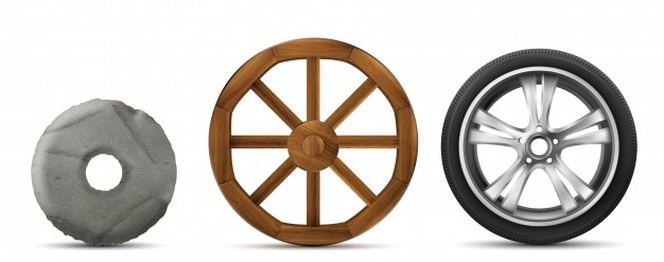
\includegraphics[width=0.79\textwidth]{img/plagiat/evolution-roue.jpg}
        \caption{
        L'évolution de la roue depuis son invention -3500 avant J.C (gauche), son allègement avec les inventions des roues à rayons en -2000 avant J.C (milieu), jusqu'aux roues à pneus en caoutchouc des véhicules que l'on utilise aujourd'hui (droite).
        }
        \label{fig:invention_roue}
    \end{figure}
\end{frame}
\begin{frame}{Simulation d'aquaplanage par Michelin}
    \begin{figure}
        \centering
        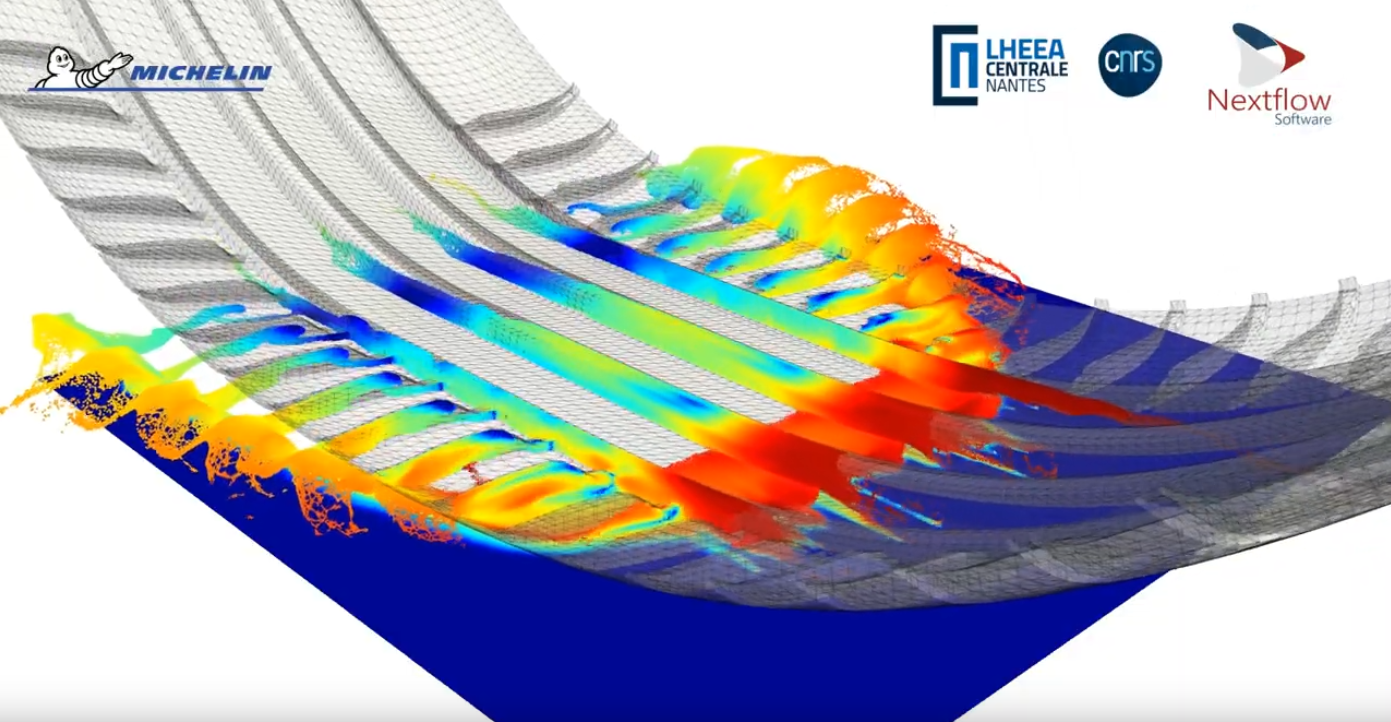
\includegraphics[width=0.79\textwidth]{img/plagiat/simulation_pneumatique_michelin.PNG}
        \caption{
            L'objectif est de s'assurer que les pneus développés par l'entreprise respectent les normes de sécurité en termes d'aquaplanage, 
            même lorsqu'ils sont usés. Image issue de \url{https://www.youtube.com/watch?v=S6csZMRy_xk}
        }
        \label{fig:simu_michelin}
    \end{figure}
\end{frame}

\iffalse
\begin{frame}{Simulation Numérique: Choix de la méthode}

    \begin{itemize}
        \item \only<1-5>{\textbf{Le modèle physique} \textcolor{darkgreen}{\footnotesize(hyperélasticité, plasticité, rupture)}}\only<6->{\textbf{Le modèle physique:} \textcolor{darkred}{\footnotesize{Choix: hyperélasticité}}}
        \item \only<2-5>{\textbf{La méthode numérique} \textcolor{darkgreen}{\footnotesize(méthode des éléments finies, différences finies, volumes finis)}}\only<6->{\textbf{La méthode numérique:} \textcolor{darkred}{\footnotesize{Choix: méthode des éléments finis}}}
        \item \only<3-5>{\textbf{La discrétisation en maillage} \textcolor{darkgreen}{\footnotesize(maillage triangulaire, quadrilatère, tétraèdrique, hexaédrique, hybride)}}\only<6->{\textbf{La discrétisation en maillage:} \textcolor{darkred}{\footnotesize{Choix: maillage quadrilatère / hexaédrique}}}
        \item \only<4-5>{\textbf{Les critères de convergence} \textcolor{darkgreen}{\footnotesize(critère de déplacement, critère de minimisation)}}\only<6->{\textbf{Les critères de convergence:} \textcolor{darkred}{\footnotesize{Choix: critère de déplacement et d'énergie sur une méthode de Newton}}}
        \item \only<5-5>{\textbf{Validation et vérification} \textcolor{darkgreen}{\footnotesize(comparaison des résultats avec des données de référence)}}\only<6->{\textbf{Validation et vérification:} \textcolor{darkred}{\footnotesize{Choix: si une simulation atteint l'itération finale, on la considère réussie}}}
    \end{itemize}

\end{frame}


\begin{frame}{Définition et propriétés fondamentales du maillage}
    \small{
        \textbf{Définition :} Un maillage $\mathcal{M}$ décompose un domaine géométrique fermé $\Omega$ en un ensemble fini d'éléments simples $(\sigma_i)_N$. 
        \begin{align*}
            \Omega = \bigcup_{0 \leq i \leq N}{\sigma_i}
        \end{align*}
    }
    \newline
    \small{
        \textbf{Conformité :} Un maillage est conforme si l'intersection entre deux éléments adjacents est vide, un sommet commun, une arête commune ou une face commune.\\
    }
    \vspace{0.5cm}
    \small{
        \textbf{Description CAO :} Représentation numérique d'un objet dans un espace 2D ou 3D utilisant des entités géométriques primitives.
    }
\end{frame}

\begin{frame}
    \frametitle{Mesh Elements}
    
    \begin{table}[]
    \centering
    \begin{tabular}{|c|c|c|}
    \hline
    & \textbf{Input} & \textbf{Output} \\ \hline
    \textbf{2D} & 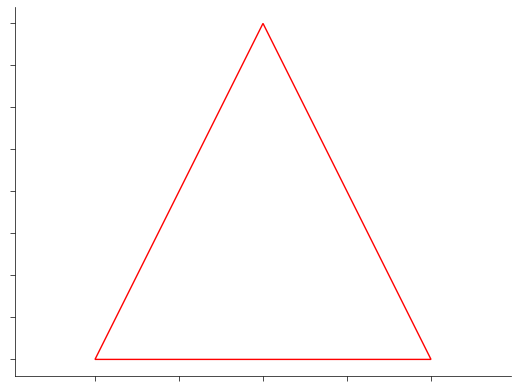
\includegraphics[width=0.2\textwidth]{img/new_images/triangle.png} & 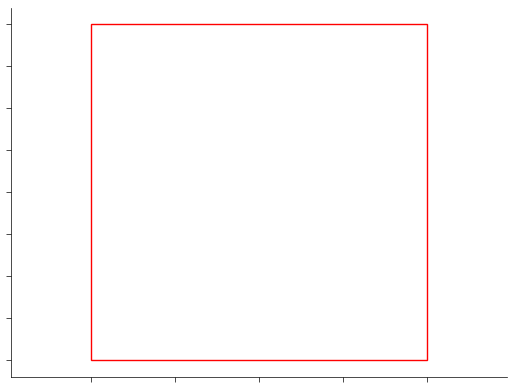
\includegraphics[width=0.2\textwidth]{img/new_images/quadrilatere.png} \\ \hline
    \textbf{3D} & 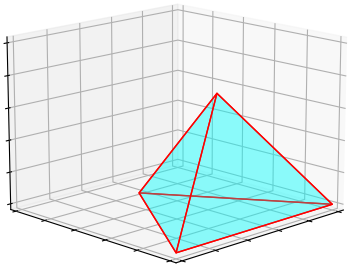
\includegraphics[width=0.2\textwidth]{img/new_images/tetrahedron.png} & 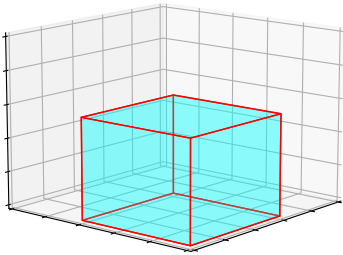
\includegraphics[width=0.2\textwidth]{img/new_images/hexahedron.png} \\ \hline
    \end{tabular}
    \end{table}
    
\end{frame}
\fi

\begin{frame}
    \frametitle{Mesh Elements}
    
    \begin{table}[]
    \centering
    \begin{tabular}{|M{1cm}|M{3cm}|M{3cm}|}
    \hline
    & \textbf{Input} & \textbf{Output} \\ [4ex] \hline
    \textbf{2D} & \raisebox{-0.5\height}{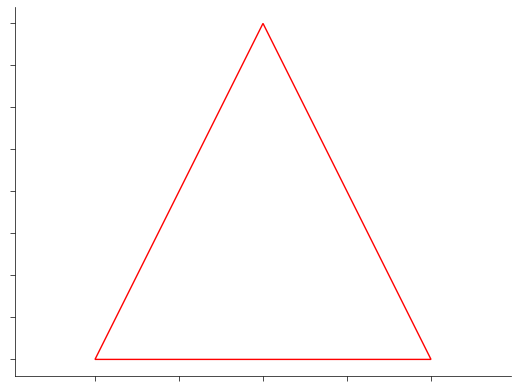
\includegraphics[width=\linewidth]{img/new_images/triangle.png}} & \raisebox{-0.5\height}{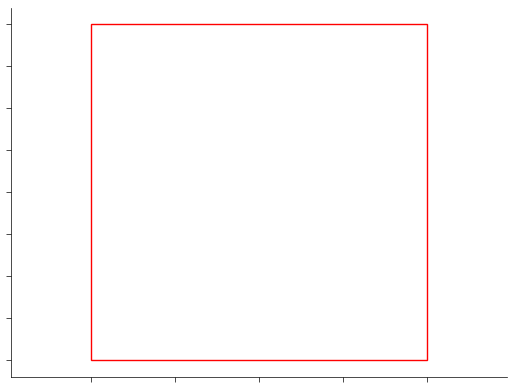
\includegraphics[width=\linewidth]{img/new_images/quadrilatere.png}} \\ [4ex] \hline
    \textbf{3D} & \raisebox{-0.5\height}{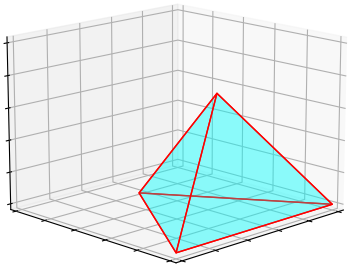
\includegraphics[width=\linewidth]{img/new_images/tetrahedron.png}} & \raisebox{-0.5\height}{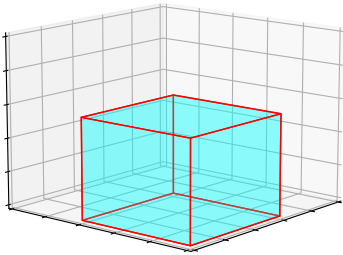
\includegraphics[width=\linewidth]{img/new_images/hexahedron.png}} \\ [4ex] \hline
    \end{tabular}
    \end{table}
    
\end{frame}

\begin{frame}{Un maillage conforme unique pour toute la simulation}
    \begin{columns}
    \column{0.5\textwidth}
    \small{
        \textbf{Objectif :} Un maillage unique pour toute la simulation, conservant une bonne qualité malgré les déformations.\\
    }
    \vspace{0.3cm}
    \small{
        \textbf{Avantage :} Les hexaèdres peuvent être déformés sans affecter leurs angles dièdres, contrairement aux tétraèdres.\\
    }
    \vspace{0.3cm}
    \small{
        \textbf{Défi :} Créer ces maillages complexes peut prendre plusieurs mois de travail ingénieur.\\
    }
    \column{0.5\textwidth}
        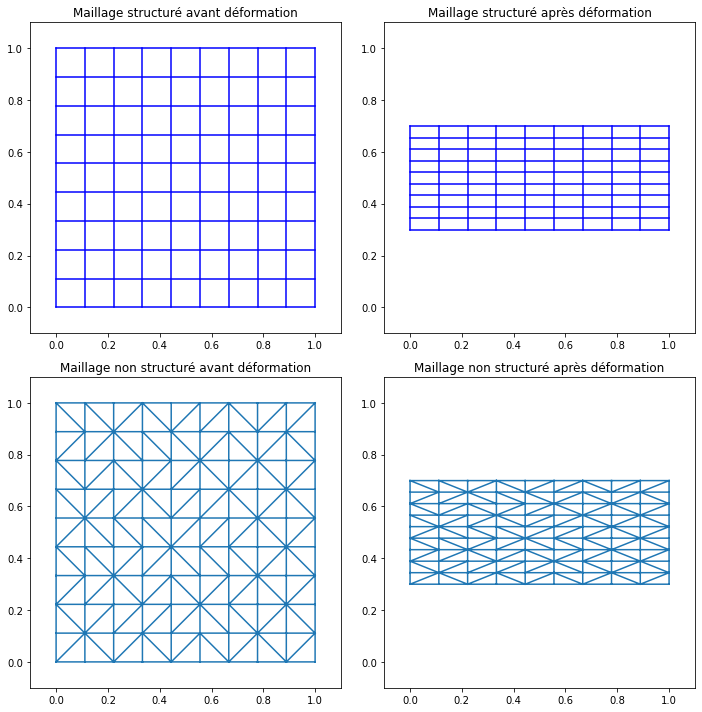
\includegraphics[width=\textwidth]{img/choix_maillage/deformation_low_angle.png}
    \end{columns}
\end{frame}


\begin{frame}{Maillage hexaédrique de qualité pour ce type de simulation}
    \small{
        \textbf{Angles dièdres :} Entre 45 et 135 degrés pour éviter les problèmes de convergence.\\
    }
    \vspace{0.5cm}
    \small{
        \textbf{Rapport d'aspect :} Maximum de 100 entre la plus grande et la plus petite arête d'un hexaèdre.\\
    }
    \vspace{0.5cm}
    \small{
        \textbf{Alignement avec les bords :} Permet de préserver la qualité des angles pendant la simulation.\\
    }
    \vspace{0.5cm}
    \small{
        \textbf{Haute qualité localisée :} Crucial dans les zones à haut gradient de force pour minimiser les erreurs numériques.\\
    }
\end{frame}